\section{Project Context}
\label{sec:problem-statement}

% =====================================================================
\subsection{Domain Context}
\label{sec:domain-context}
Smartphones have become the default place to fill the small gaps of a day:
the minutes between classes, on a bus, or between two tasks at work. Music,
news and short videos are popular ways to fill those gaps, and many of the
services that provide them are designed to maximise engagement. Infinite
scrolling, autoplay and algorithmic feeds remove natural stopping points, so a
break that was meant to last a few minutes can quietly grow into a much longer
period of unplanned screen time. The scale of this behaviour is large.
According to the Digital 2026 Global Overview Report, online adults spend an
average of 18 hours and 36 minutes per week, which is well over two and a half
hours per day, scrolling social and video feeds, and 39.7 percent of adult
social media users say that filling spare time is one of their main reasons
for using these platforms~\cite{kemp2025digital2026}.

\begin{figure}[H]
  \centering
  \begin{subfigure}{0.40\textwidth}
    \centering
    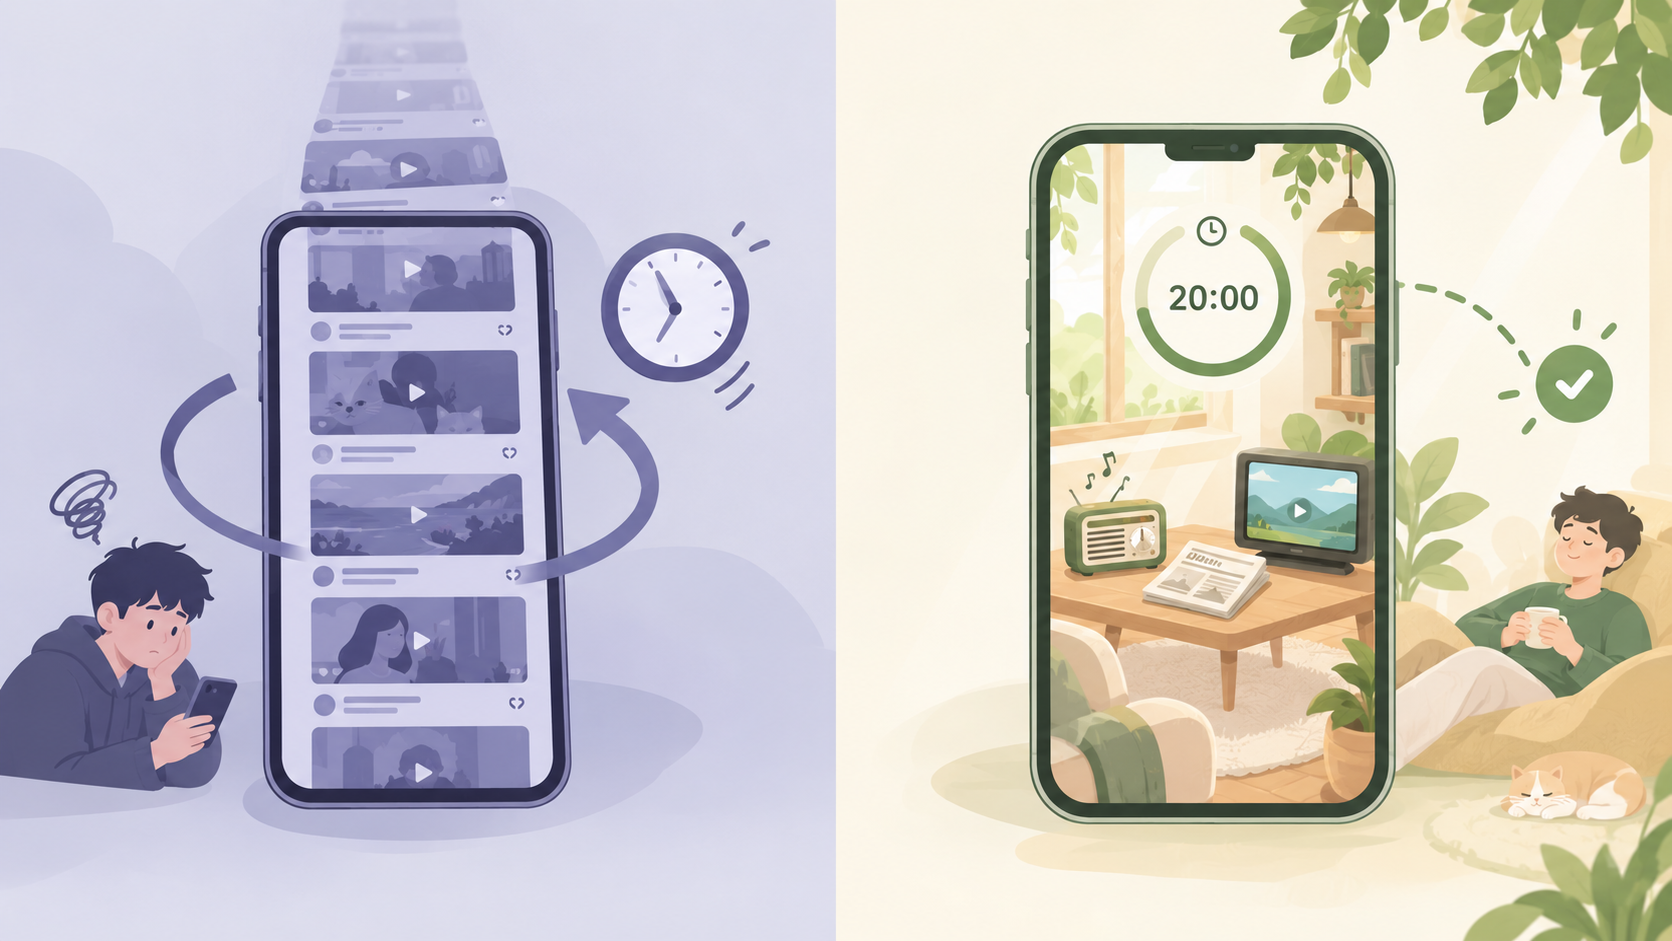
\includegraphics[width=\linewidth]{graphics/bia/1/phone.png}
  \end{subfigure}\hspace{1.5em}
  \begin{subfigure}{0.40\textwidth}
    \centering
    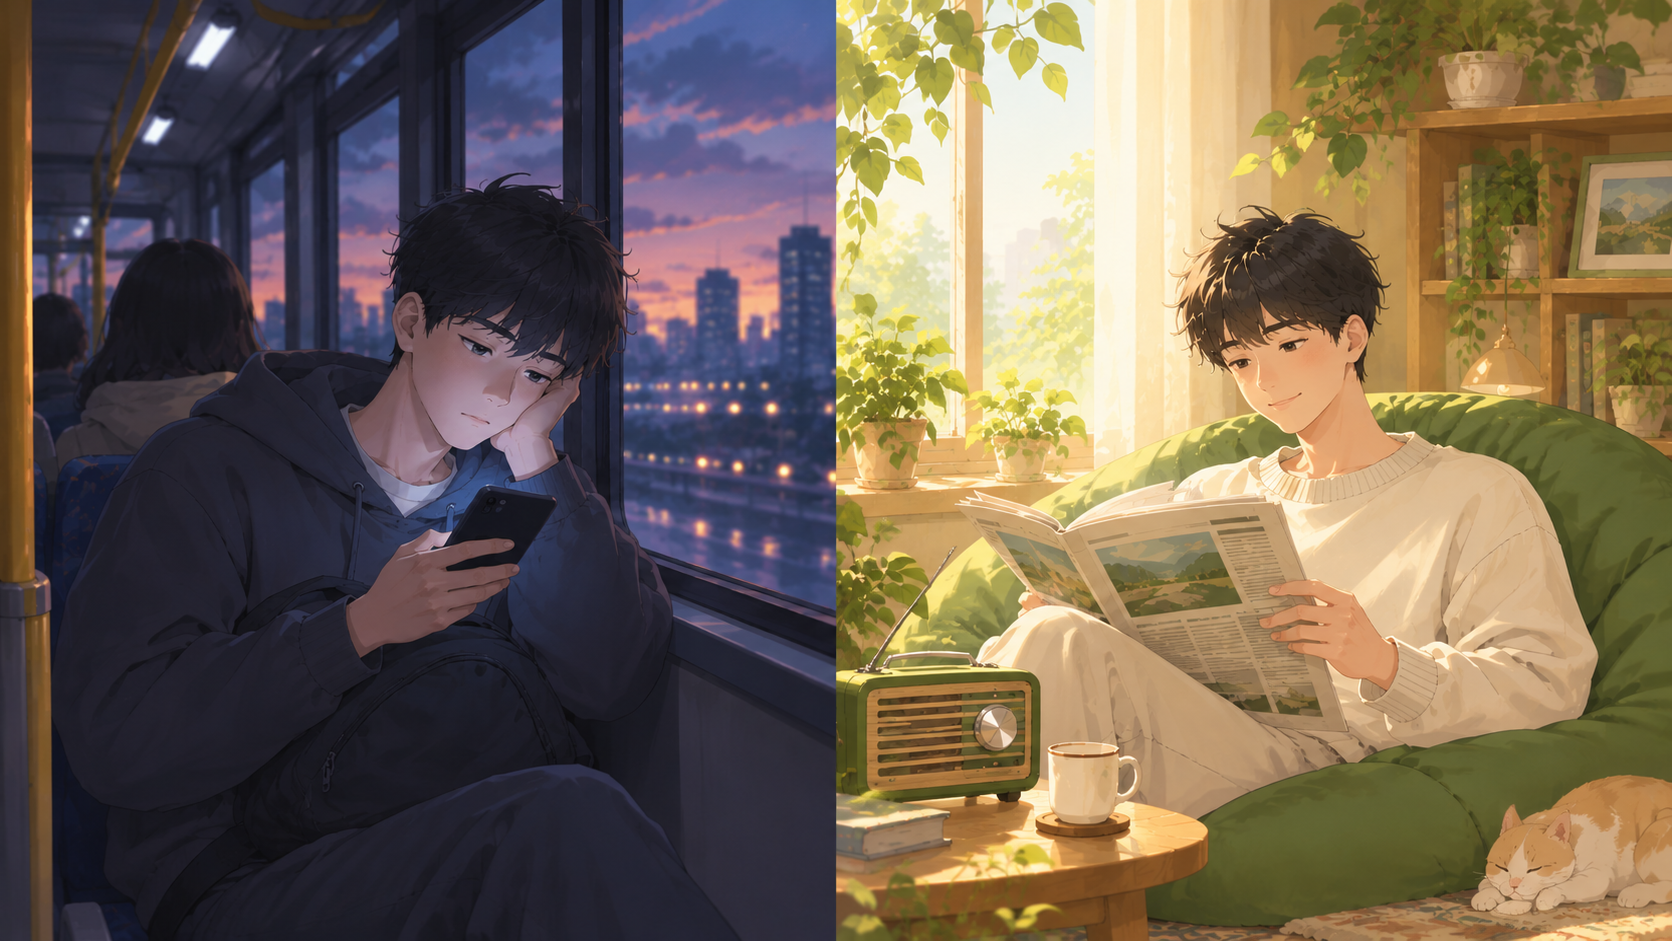
\includegraphics[width=\linewidth]{graphics/bia/1/moods.png}
  \end{subfigure}
  \caption{Illustration of 2 kinds of spare-time moments: a short break between tasks and a doomscrolling session.}
  \label{fig:space-themes}
\end{figure}

At the same time, digital wellbeing has become a visible concern for users and
platform vendors. Screen-time dashboards, app timers and focus modes are now
common, but most of them work by restricting access. Few offer something
enjoyable to do within a limit. This gap is where Breakly operates: in the
domain of mobile entertainment, as an app whose central feature is a stopping
point, designed for exactly those spare-time moments. The domain is treated
purely as an interaction-design and product problem; the project makes no
medical or clinical claims.

Breakly addresses this gap through four core ideas that recur throughout this
document. A time-boxed session is a period of 10, 20 or 30 minutes chosen by
the user, with a visible countdown and an automatic end. Finite content means
that every feed has an end, for example a limited list of short videos
followed by an end card. The Space is a calm illustrated scene whose objects
(a radio, a newspaper and a television) open the music, news and video
services, and the scene can be switched between themes. Finally, a streak is
the number of consecutive days with at least one completed session.


% =====================================================================
\subsection{Related Apps}
\label{sec:related-apps}

To position Breakly, we reviewed six apps and compared them on content
offered, session and time controls, finite-content design, and visual
experience. The apps were selected into two groups.The SWOT tables below are the team's assessment based on store listings and
hands-on use.

% ---------------------------------------------------------------------
\subsubsection{Direct Competitors}
\label{sec:direct-competitors}
Direct competitors are apps that users already open for the same purpose as Breakly: a quick, enjoyable break with music, news or short video.

\paragraph{YouTube (including Shorts).}
A general video platform offering long-form videos, Shorts, music videos and
news channels.

\begin{figure}[H]
  \centering
  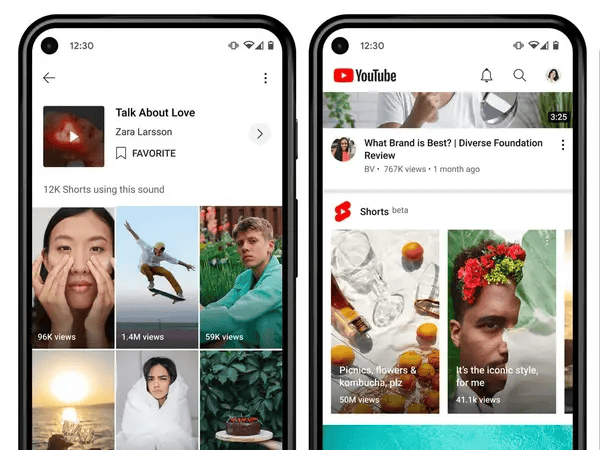
\includegraphics[width=0.5\textwidth]{graphics/bia/1/youtube.png}
  \caption{YouTube interface used for comparison}
  \label{fig:app-youtube}
\end{figure}

\appswot{YouTube}{youtube}
  {\item Huge and varied library covering video, music and news
   \item Strong search and recommendations
   \item Available on every major platform}
  {\item Autoplay and recommendations keep users watching
   \item Break reminders are optional and easy to ignore
   \item No concept of a bounded session}
  {\item Becoming a one-stop entertainment hub
   \item Users already trust it for news and music}
  {\item Strong competition from other short-video apps
   \item Changes in advertising and content policies}

\paragraph{Spotify.}
A music and podcast streaming service with personalised playlists and a
sleep timer.

\begin{figure}[H]
  \centering
  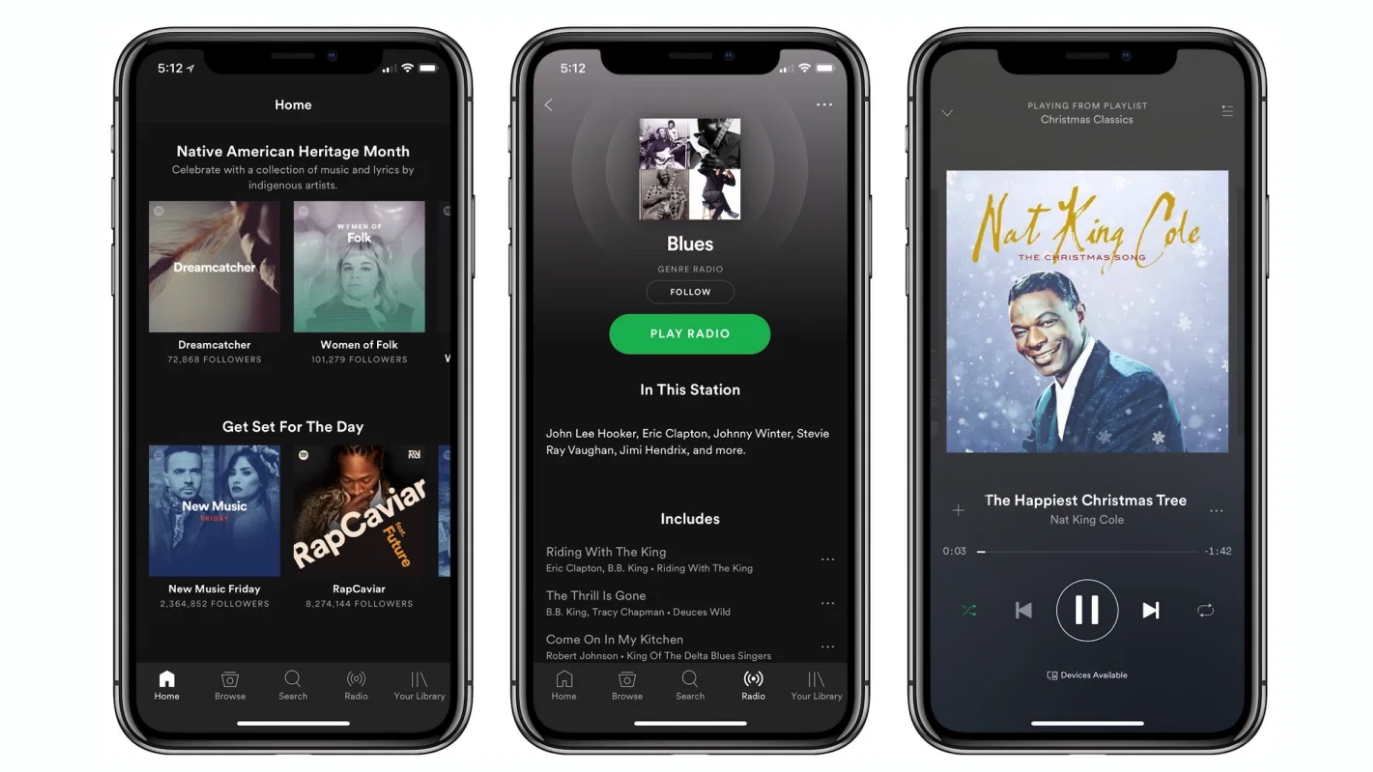
\includegraphics[width=0.85\textwidth]{graphics/bia/1/spotify.png}
  \caption{Spotify interface used for comparison}
  \label{fig:app-spotify}
\end{figure}

\appswot{Spotify}{spotify}
  {\item Very large music catalogue
   \item Strong personalisation and mood or focus playlists
   \item Reliable background and lock-screen playback}
  {\item Audio-centred, with little reading or video content
   \item Some playback features are limited on the free tier
         \textbf{[verify]}
   \item No limit on the overall entertainment session}
  {\item High interest in focus and chill playlists
   \item Room to extend into more content types}
  {\item Licensing costs and rivalry from other streaming platforms
   \item Users may switch to free video platforms for music}

\paragraph{VnExpress.}
One of the most widely read Vietnamese online newspapers, available as a
website and a mobile app, with an English edition (VnExpress International).
It covers current affairs, business, sports, culture and other categories
with text, photos and video \textbf{[verify]}.

\begin{figure}[H]
  \centering
  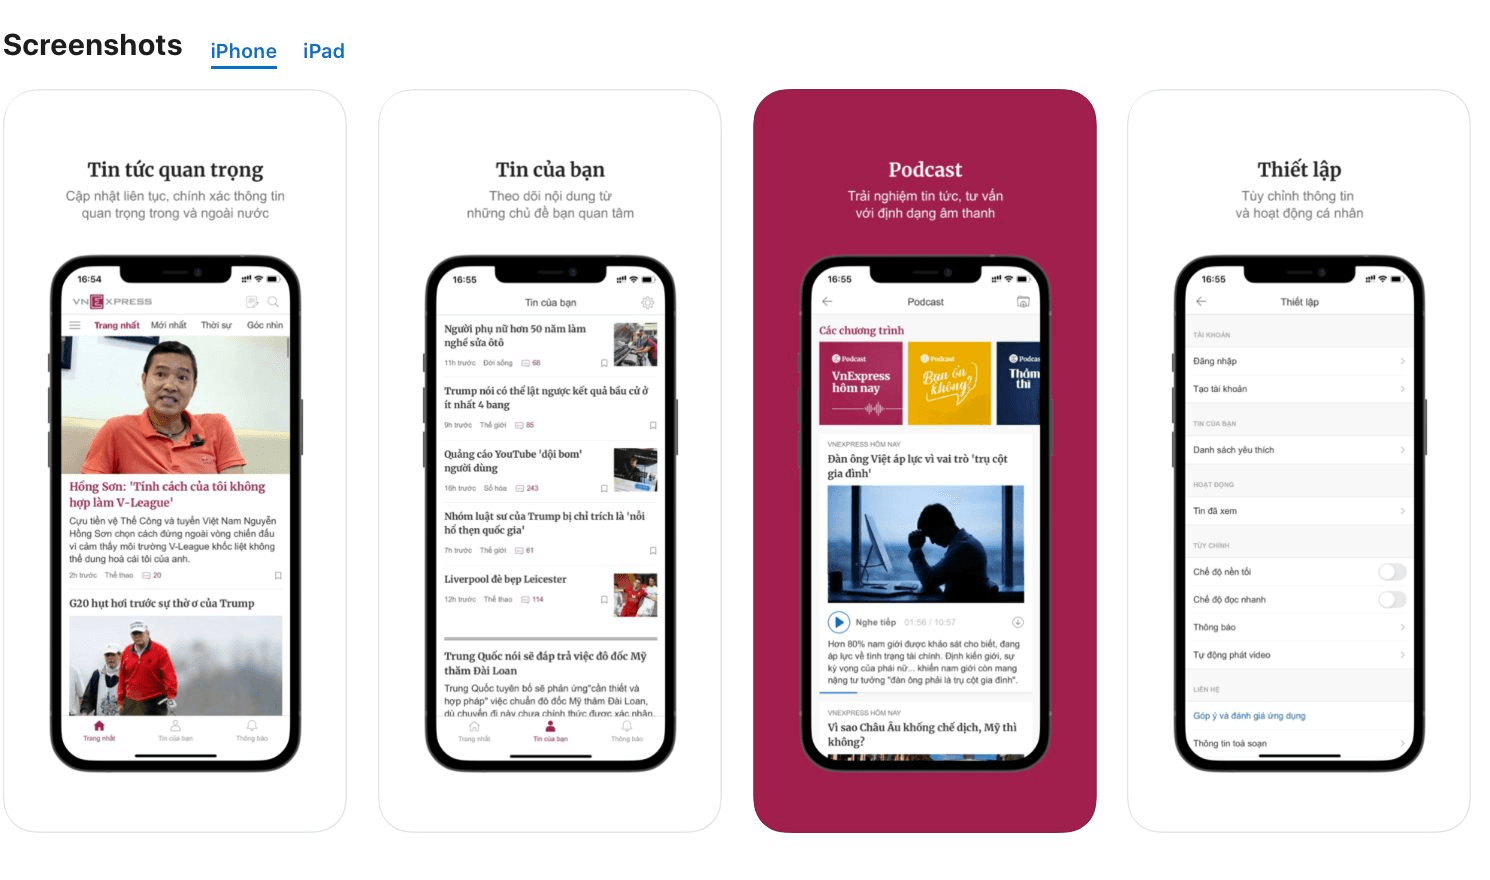
\includegraphics[width=0.85\textwidth]{graphics/bia/1/vnexpress.png}
  \caption{VnExpress interface used for comparison}
  \label{fig:app-vnexpress}
\end{figure}

\appswot{VnExpress}{vnexpress}
  {\item Broad, up-to-date coverage from an established newsroom
   \item Clear category navigation
   \item Familiar and trusted among Vietnamese readers}
  {\item Reading-only experience, with no music or relaxation layer
   \item Long lists of related stories make it easy to keep reading with no
         natural stopping point \textbf{[verify]}
   \item No awareness of how much time the reader has}
  {\item Growing demand for short, easy-to-digest news
   \item English edition reaches international readers}
  {\item Readers increasingly get news through social and short-video platforms
   \item Competition from many other news apps and aggregators}

% ---------------------------------------------------------------------
\subsubsection{Indirect Competitors}
\label{sec:indirect-competitors}
Indirect competitors address the underlying need, which is taking more controlled and restorative breaks or reducing overuse, but through timers, blocking or relaxation content rather than general entertainment.

\paragraph{Forest.}
A focus timer in which a virtual tree grows while the user stays away from
the phone.

\begin{figure}[H]
  \centering
  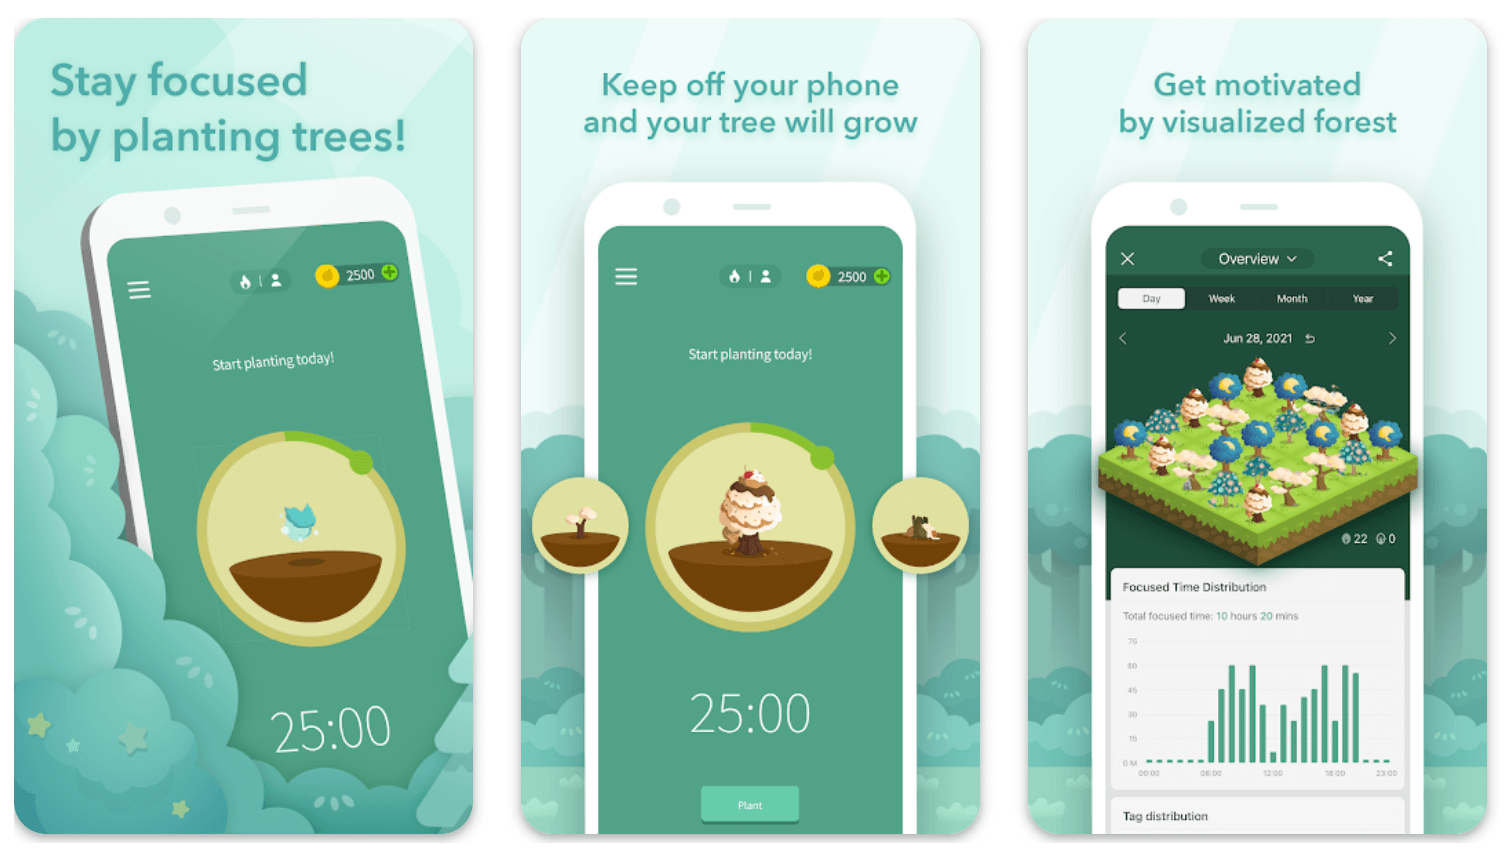
\includegraphics[width=0.85\textwidth]{graphics/bia/1/forest.png}
  \caption{Forest interface used for comparison}
  \label{fig:app-forest}
\end{figure}

\appswot{Forest}{forest}
  {\item Simple and motivating gamification
   \item Clear start, end and visual progress}
  {\item Provides no entertainment for the break itself
   \item Built to avoid the phone rather than to improve a break}
  {\item Strong demand for focus and study tools among students}
  {\item Many free alternatives and built-in focus modes}

\paragraph{Opal (screen-time and app-blocking tools).}
An app that blocks distracting apps for set periods and reports phone usage.

\begin{figure}[H]
  \centering
  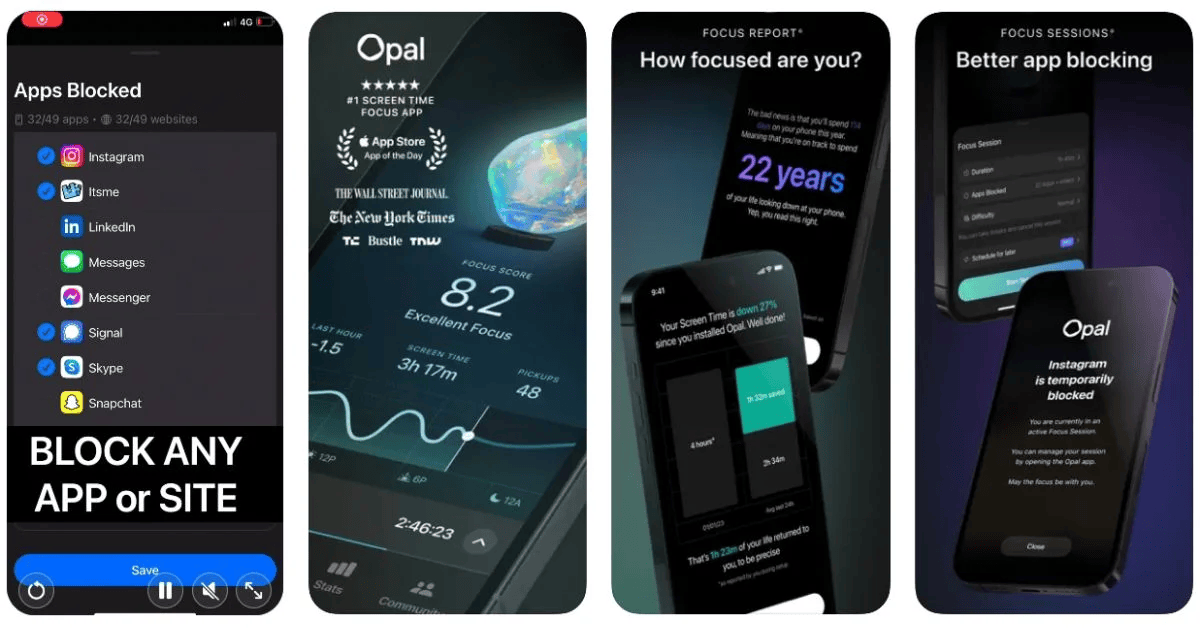
\includegraphics[width=0.85\textwidth]{graphics/bia/1/opal.png}
  \caption{Opal interface used for comparison}
  \label{fig:app-opal}
\end{figure}

\appswot{Opal}{opal}
  {\item Effective at restricting access to distracting apps
   \item Usage reports that make habits visible}
  {\item Restrictive rather than rewarding
   \item Offers no alternative content
   \item Limits can be switched off by the user}
  {\item Rising awareness of screen time and digital wellbeing}
  {\item Free built-in operating system features (Screen Time, Digital
         Wellbeing) cover similar needs}

\paragraph{Calm.}
A relaxation app with guided sessions, sleep stories, music and nature
sounds.

\begin{figure}[H]
  \centering
  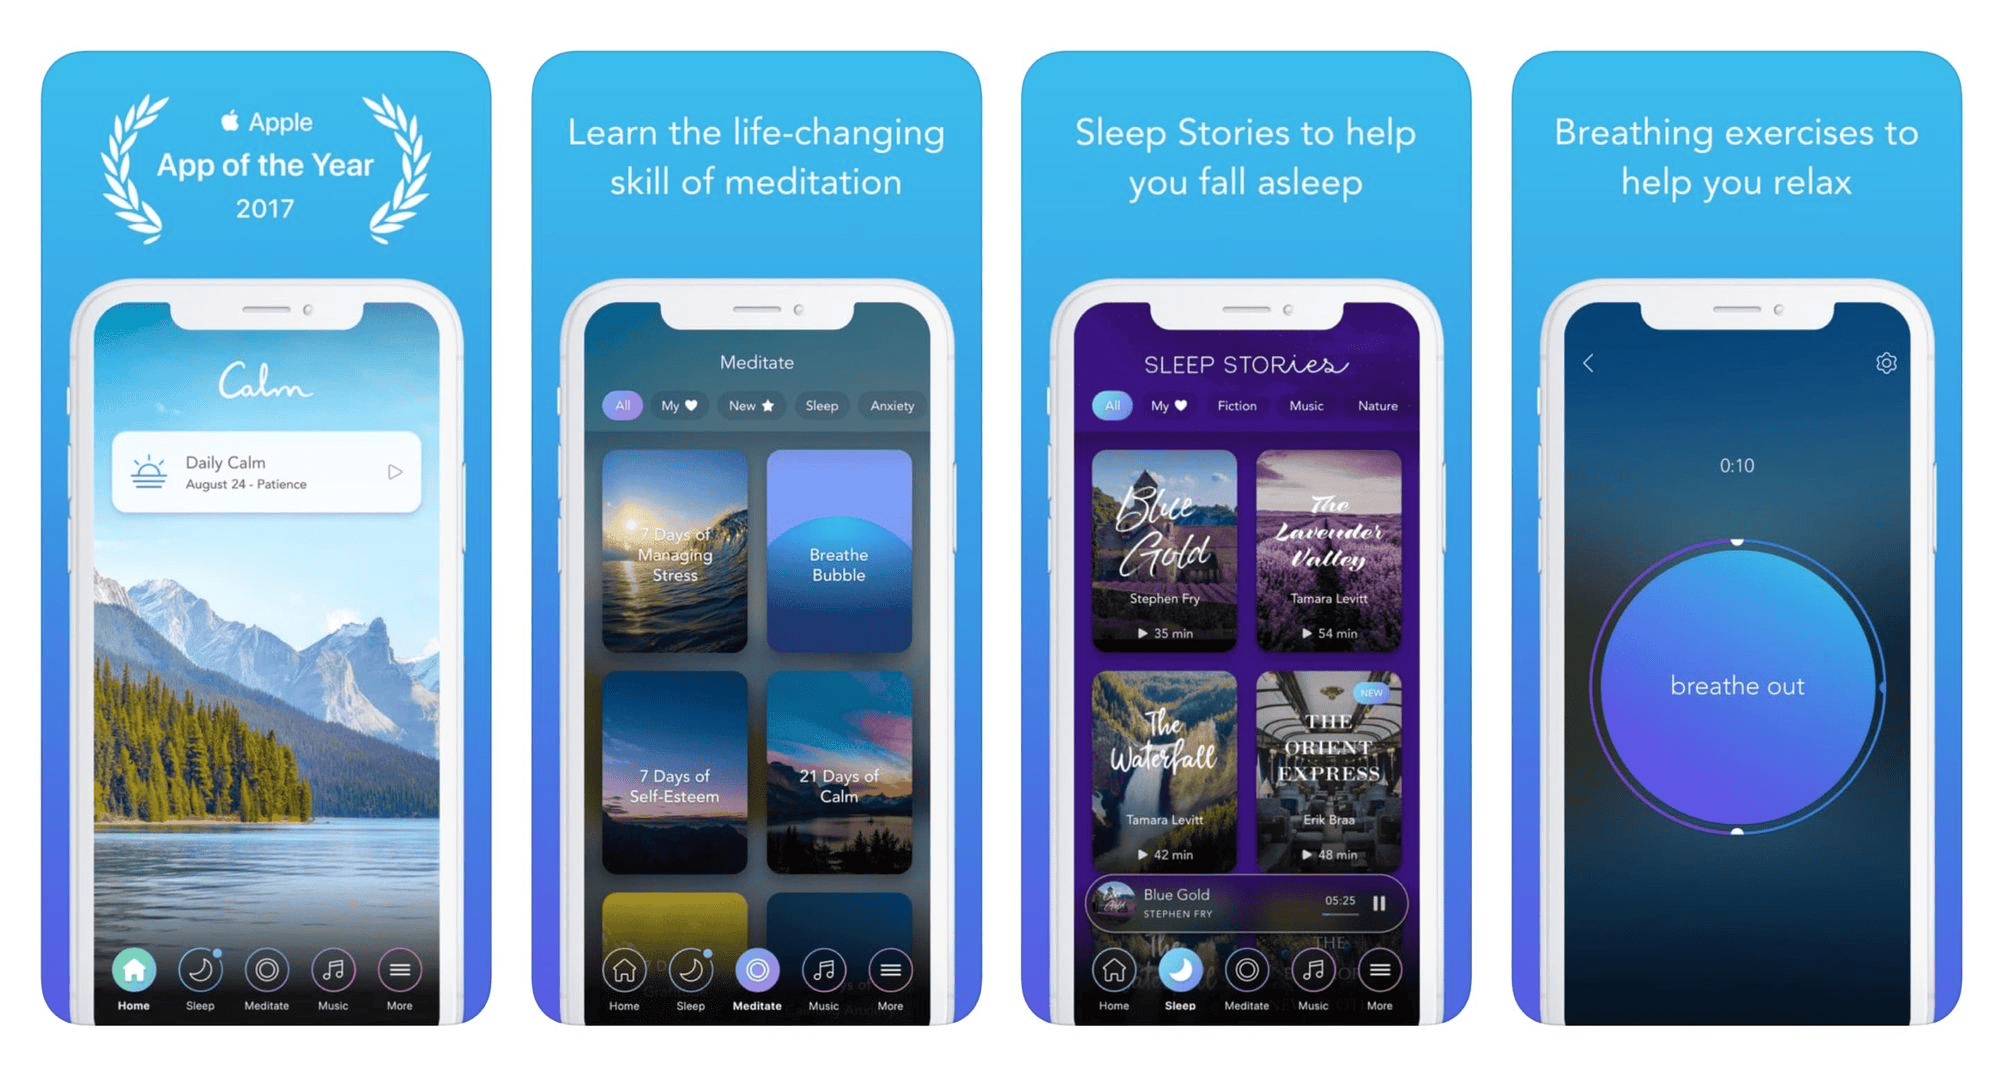
\includegraphics[width=0.85\textwidth]{graphics/bia/1/calm.png}
  \caption{Calm interface used for comparison}
  \label{fig:app-calm}
\end{figure}

\appswot{Calm}{calm}
  {\item Polished and soothing experience
   \item High-quality audio content and calming visuals}
  {\item Wellness-focused, with no news or short video
   \item Much of the content is behind a subscription \textbf{[verify]}}
  {\item Growing interest in wellbeing and mindfulness}
  {\item Free alternatives such as relaxation videos and playlists on general platforms}

% ---------------------------------------------------------------------
\subsubsection{Feature Comparison}
\label{sec:feature-comparison}

\begin{longtable}{|p{3.3cm}|*{7}{p{1.2cm}|}}
\caption{Feature comparison of the reviewed apps ($\checkmark$ supported,
         $\circ$ partial or optional, $-$ not offered, n/a not applicable;
         \textbf{to be verified against current app versions})}
\label{tab:feature-comparison}\\
    \hline
    \textbf{Feature} & \textbf{YouTube} & \textbf{Spotify} & \textbf{VnExpress}
      & \textbf{Forest} & \textbf{Opal} & \textbf{Calm} & \textbf{Breakly} \\
    \hline
\endfirsthead
\multicolumn{8}{r}{\textit{Continued from previous page}}\\[-2pt]\hline
\textbf{Feature} & \textbf{YouTube} & \textbf{Spotify} & \textbf{VnExpress}
  & \textbf{Forest} & \textbf{Opal} & \textbf{Calm} & \textbf{Breakly} \\
\hline
\endhead
\multicolumn{8}{r}{\textit{Continue on next page}}\\
\endfoot
\endlastfoot
    Music & $\circ$ & $\checkmark$ & $-$ & $-$ & $-$ & $\checkmark$ & $\checkmark$ \\ \hline
    News and reading & $\circ$ & $-$ & $\checkmark$ & $-$ & $-$ & $-$ & $\checkmark$ \\ \hline
    Short video & $\checkmark$ & $\circ$ & $\circ$ & $-$ & $-$ & $-$ & $\checkmark$ \\ \hline
    Built-in session length & $\circ$ & $\circ$ & $-$ & $\checkmark$ & $\checkmark$ & $\circ$ & $\checkmark$ \\ \hline
    Finite content by design & $-$ & $-$ & $-$ & n/a & n/a & $\circ$ & $\checkmark$ \\ \hline
    Themed immersive environment & $-$ & $-$ & $-$ & $\circ$ & $-$ & $\circ$ & $\checkmark$ \\ \hline
\end{longtable}

Based on the apps reviewed, general entertainment apps supply content but no
stopping point, while focus and wellbeing tools supply limits but little
enjoyable content. Breakly aims to occupy the gap between them: entertaining
content inside a bounded, calm session.

% ---------------------------------------------------------------------
\subsubsection{SWOT Analysis of Breakly}
\label{sec:swot-breakly}

The competitor review is summarised in a SWOT analysis of Breakly itself
(Table~\ref{tab:swot-breakly}). Its items are referenced by code (S1, W2,
and so on) in the system overview.

\noindent\textbf{Table: SWOT analysis of Breakly}\label{tab:swot-breakly}\par
  \swotbox
    {\item \textbf{S1} Finite by design: every session and video feed has a clear end
     \item \textbf{S2} Music, news and short video in one calm Space, reachable in two taps
     \item \textbf{S3} Swappable themes add emotional appeal without changing the interface
     \item \textbf{S4} Achievable scope for a two-person team using one cross-platform codebase}
    {\item \textbf{W1} Content depends on third-party sources whose terms may limit usage
     \item \textbf{W2} Small catalogue and no personalised recommendation compared with large platforms
     \item \textbf{W3} Most content needs a network connection}
    {\item \textbf{O1} Growing public concern about screen time and endless feeds
     \item \textbf{O2} Students and young professionals have many short breaks every day
     \item \textbf{O3} Streaks, history and new Spaces can build a habit and extend the product later}
    {\item \textbf{T1} Large platforms may add stronger break and limit features
     \item \textbf{T2} Strong existing habits around YouTube and other short-video platforms
     \item \textbf{T3} Changes in licence or API terms could remove content sources}

% =====================================================================
\subsection{System Overview}
\label{sec:system-overview}

Breakly is a mobile application that turns a short entertainment break into
a time-boxed session. The user states how much free time they have (10, 20
or 30 minutes) and enters a calm illustrated Space. Three objects in the
Space open the services: a radio for background music, a newspaper for news
and a television for a finite feed of short videos. A countdown stays
visible while the user enjoys the content. When time is up, the session ends
automatically, a short summary is shown and the user's daily streak is
updated.

The system is made of four parts. The first is a cross-platform mobile client
built with React Native and Expo, which contains the session engine (timer
and session state), the Space and theme layer, and the screens for music,
news, video, history and settings. The second is a managed backend
\textbf{[TODO: Supabase or Firebase]} that provides authentication and stores
session history, streaks and preferences. The third is a set of external
content services: news from RSS feeds, music from an openly licensed
catalogue and short videos from a video API \textbf{[TODO: select the sources
and verify their terms]}. The fourth is local storage on the device for
preferences, cached content and session state, so that the countdown stays
correct and recent history can still be shown when the connection drops,
although playing music, news and video requires a network connection.

The design follows three pillars, each responding to the SWOT analysis in
Table~\ref{tab:swot-breakly}.

The first pillar is User Experience. A session starts in two taps from the
Home Space, the countdown is visible on every screen and stays accurate when
the app is in the background, and video feeds are finite and end with a clear
end card. Themes change the look of the Space but never its layout or
behaviour, and the main screens are targeted to load within three seconds
under normal network conditions \textbf{[TODO: confirm the figure in the
non-functional requirements]}. This pillar preserves the strengths S1 to S3
and is the main answer to the threats T1 and T2: Breakly cannot win on
content volume, so it must win on experience.

The second pillar is Security \& Privacy. Sign-in is handled by a managed
authentication service and access tokens are kept in secure device storage.
The app collects only account details, session history and preferences, does
not request location or contacts, and includes no advertising trackers. The
notification permission is requested only after a short explanation, when
the user turns on a reminder. Using official feeds and APIs with clear terms,
and showing content credits, reduces the weakness W1 and the threat T3.

The third pillar is Business Goals. Retention comes from streaks and session
history that reward regular, controlled breaks, and new Spaces can be added
without redesigning the interface, which keeps the product extendable (O3).
The growing concern about screen time (O1) gives the product a clear reason
to exist. Content sources are chosen for clear licence terms. Within the
course, the goal is a reliable, demonstrable MVP that implements all
Must-have requirements; any paid features, such as premium Spaces, are out of
scope.

Weakness W3 (network dependency) is addressed through explicit loading,
offline and error states on every content screen, and weakness W2 is accepted
as a deliberate trade-off: a small, well-curated catalogue is consistent with
the idea of finite entertainment.

% =====================================================================
\subsection{Stakeholders}
\label{sec:stakeholders}

\begin{longtable}{|p{3.2cm}|p{0.31\textwidth}|p{0.43\textwidth}|}
\caption{Initial stakeholder analysis}\label{tab:stakeholders}\\
\hline
\textbf{Stakeholder} & \textbf{Interest} & \textbf{Project implication} \\
\hline
\endfirsthead
\multicolumn{3}{r}{\textit{Continued from previous page}}\\[-2pt]\hline
\textbf{Stakeholder} & \textbf{Interest} & \textbf{Project implication} \\
\hline
\endhead
\multicolumn{3}{r}{\textit{Continue on next page}}\\
\endfoot
\endlastfoot
Students and young professionals (end users) & Enjoy a short break that
they can stop on time & Two-tap start, visible timer, finite content, and a
calm, accessible interface. \\
\hline
Content providers (news publishers, music and video platforms) & Their
content is used within their licence and terms & Use official feeds and
APIs, show source credits, and respect usage limits. \\
\hline
Platform and service providers (backend service, Expo, app stores) &
Service terms, quotas and store policies are respected & Stay within quota
limits and follow store guidelines and permission rules. \\
\hline
Project team & Deliver a reliable mobile MVP & Testable requirements and
measurable quality targets. \\
\hline
Course instructor and evaluators & Assess usability, completeness, and
technical quality & Traceable evidence and reproducible demonstrations. \\
\hline
\end{longtable}

% =====================================================================
\subsection{Personas}
\label{sec:personas}

The three personas below are provisional. Values marked ``assumed'' reflect
the team's expectations and will be validated or corrected with the survey
and interview results \textbf{[TODO: add a reference to the elicitation
section]}.

\subsubsection{Linh -- The Overloaded Student}

Linh is a university student who studies in long sessions and opens
short-video apps ``for five minutes'' that often turn into an hour. She wants
a break that refreshes her and that she can stop on time.

\persona{Persona 1: Linh, the overloaded student}{tab:persona-linh}
  {\item Age 21, full-time university student
   \item Lives in Ho Chi Minh City, Vietnam
   \item High tech-savviness; comfortable with many apps}
  {\item Take a short, enjoyable break between study blocks
   \item Stay in control of how long the break lasts
   \item Start quickly, with one hand, without setting anything up}
  {\item Loses track of time on short-video feeds and feels guilty afterwards
   \item Focus timers give her no enjoyable content during the break
   \item Break reminders that interrupt her work}
  {\item Android phone (assumed)
   \item About 5 to 6 hours of screen time per day (assumed)
   \item Uses the phone on the bus, between classes and in cafes; often
         one-handed and with earphones; mobile data or public Wi-Fi}

\subsubsection{Minh -- The Desk-Based Professional}

Minh works at a computer and wants a predictable ten-to-twenty-minute reset
between meetings or during lunch. He likes background music while reading the
news, and does not want to juggle several apps to do it.

\persona{Persona 2: Minh, the desk-based professional}{tab:persona-minh}
  {\item Age 27, office worker at a company
   \item Lives in Ho Chi Minh City, Vietnam
   \item Medium to high tech-savviness}
  {\item Reset his mind in a fixed, short window
   \item Read the news with music in the background
   \item Resume or skip an activity without losing track of time}
  {\item Switches between a music app, a news app and a video app
   \item News apps feel cluttered and breaks overrun into work time
   \item Hard to find something calm that fits a 10-minute gap}
  {\item iPhone (assumed)
   \item About 4 to 5 hours of screen time per day (assumed)
   \item Uses the phone at his desk, at lunch and on his commute; reliable
         office Wi-Fi, mobile data when travelling; earphones in shared
         spaces}

\subsubsection{An -- The Accessibility-Conscious User}

An prefers larger text and high-contrast interfaces. An needs readable
content, sufficiently large touch targets, and timer feedback that is not
communicated by colour alone.

\persona{Persona 3: An, the accessibility-conscious user}{tab:persona-an}
  {\item Age 34, freelance writer working from home
   \item Lives in Hanoi, Vietnam
   \item Medium tech-savviness; relies on system accessibility settings}
  {\item Enjoy music and news in a comfortable, readable interface
   \item Know exactly how much time is left at a glance
   \item Use simple, predictable controls}
  {\item Small text and low contrast in many entertainment apps
   \item Tiny touch targets and controls that are easy to miss
   \item Timers and alerts that rely on colour alone}
  {\item Android phone with a larger system font size (assumed)
   \item About 3 to 4 hours of screen time per day (assumed)
   \item Mostly indoors at home, on Wi-Fi; uses the phone for short breaks
         between writing sessions}